\section{Extension of the Capra solution}\label{sec:extension}
\sideboxbegin{o}
This section depicts what has been changed in Capra to foster trace quality. It details the new features and their benefits, as well as the potential impact such changes may propagate.
\sideboxend

Depending on the purpose, the entities used by Trace\textit{a} will have stronger or lesser interest. If the purpose is to find who is responsible for a bug, the agency might be the most salient element of the project to understand who's run what and what triggered who. Yet, if the purpose is to locate the bug, the granularity of the artefacts and the uncertainty of the identification process will be of greater importance. The integration of Trace\textit{a} into Capra allows both - and more.


We first introduce in this section the integration of Trace\textit{a} into Capra and the changes we applied.
The implementation of such changes impacts the quality of the overall Capra solution. We depict these concerns as well as limitations that could not be addressed.



\subsection{Integration of Trace\textit{a}}
We address the lack of quality assessment of trace elements by hacking the customization mechanism of Capra. We integrate Trace\textit{a}, our metamodel for traceability \cite{batot2021-not-another-metamodel}, into Capra as a custom metamodel\footnote{As explained in \url{https://wiki.eclipse.org/Capra/CustomTraceabilityMetaModel}}. We adapted Trace\textit{a} to fit with Capra's requirements and translated it as an XCore project. 

\begin{descriptioncompact}
    \item[1 -- Add trace quality to Capra's metamodel] 
    \item[2 -- Extend Capra's core interface]
    \item[3 -- Augment Capra's user experience]
\end{descriptioncompact}

\subsubsection{Trace model, relationships, and agency}
As can be seen in Listing \ref{lst:traces}, at the root of the Ecore model, a trace model is defined with links and agents. All concepts (except for the model) derive from \texttt{TracingElement}. They have a unique ID and a time stamp. They may also refer to which agent is responsible for their creation. An \texttt{Agent} may be a human being (\texttt{HumanAgent}) or a piece of machinery (\texttt{MachineAgent}).
The type of the relationships is either a \texttt{DomainLink} or a \texttt{EngineeringLink} depending if the link represent a relationship in the realm of the model or the one of the modeler, respectively. 

\begin{center}
\begin{lstlisting}[caption={Confidence and evidences for trustable traceability},label=lst:relationship,style=mystylextext,frame=shadowbox, rulesepcolor=\color{blue}]
Relationship  returns SysML::Relationship :
    'relationship' Identification?
    RelationshipRelatedElements
    RelationshipBody;

OwnedRelationship returns SysML::Relationship :
    'relationship' Identification?
    'to' RelationshipTargetList
    RelationshipBody;

fragment RelationshipRelatedElements 
            returns SysML::Relationship :
    'from' RelationshipSourceList ( 'to' RelationshipTargetList )?
  | 'to' RelationshipTargetList;

fragment RelationshipSourceList returns SysML::Relationship :
    RelationshipSource ( ',' RelationshipSource )*;

fragment RelationshipSource returns SysML::Relationship :
    source += [SysML::Element | QualifiedName];

fragment RelationshipTargetList returns SysML::Relationship :
    RelationshipTarget ( ',' RelationshipTarget )*
;

fragment RelationshipTarget returns SysML::Relationship :
    target += [SysML::Element | QualifiedName];

fragment RelationshipBody returns SysML::Relationship :
    ';' | '{' RelationshipOwnedElement* '}';

fragment RelationshipOwnedElement returns SysML::Relationship:
      ownedRelatedElement += OwnedRelatedElement
    | ownedRelationship += OwnedDocumentation
    | ownedRelationship += OwnedTextualRepresentationAnnotation;

OwnedRelatedElement returns SysML::Element :
      'element' ( humanId = Name )? ElementBody
    | OwnedRelatedRelationship;

OwnedRelatedRelationship returns SysML::Relationship :
    'relationship' ( humanId = Name )? RelationshipBody;
\end{lstlisting}
\end{center}


To integrate the new link types and link attributes to Capra, the API of  \verb|org.eclipse.capra-| \verb|.generic.tracemodel.GenericMetaModelAdapter| must be adapted (see Listing \ref{lst:timapi}). We defined here generic methods to browse  links and and their origins and targets. Everything is configurable. As long as new link types derive from \texttt{RelatedTo}, they will be augmented with quality attributes (\ie confidence and evidence).
In the same manner, class \verb|org.eclipse.capra.generic.tracemodel.AbstractMetaModelAdapter| offers an interface to define how \textit{internal traces} (\ie~links inside traced elements) must be handled. 
%org.eclipse.capra.core.adapters.TraceMetaModelAdapter



\begin{lstlisting}[caption={AbstractMetaModelAdapter interface},
label=lst:timapi2,
style=mystylexcore,
frame=shadowbox, 
rulesepcolor=\color{blue},
morekeywords={class,contains,abstract,extends,\{,\},\[,\],refers,derived,String,get,int,double,List,Connection,EObject,void,String,boolean,Collection,EClass},
linewidth=17.5cm,
xleftmargin=0.3cm
]
void deleteTrace(List<Connection> toDelete, EObject traceModel);
List<Connection> getInternalElements(EObject element, EObject traceModel, 
    List<String> traceLinkTypes);
List<Connection> getInternalElementsTransitive(EObject element, 
    EObject traceModel, List<String> traceLinkTypes, int transitivityDepth);
boolean isThereAnInternalTraceBetween(EObject first, EObject second);
\end{lstlisting}








\subsubsection{Trace confidence and explainability}
Listing \ref{lst:quality}, represents the \texttt{Confidence} value (\ie an estimation of the existence of the link). Trace\textit{a} define classes for the different kinds of evidences that may testify the value of the confidence. An \texttt{Evidence} can be a textual annotation (\texttt{Annotation-Evidence}), or a \texttt{RuleEvidence} when a link is created automatically, or an \texttt{AIEvidence} when a learning algorithm is used to identify the link. These latter possess attributes to reproduce their execution (\eg the rule, a certain kind of algorithm, the training set used).


%\begin{center}
\begin{lstlisting}[caption={Confidence and evidences for trustable traceability},label=lst:quality,style=mystylexcore,frame=shadowbox, rulesepcolor=\color{blue}]
class Confidence extends TracingElement {
	contains Evidence [0..1] evidence
	double value 
}

abstract class Evidence  extends TracingElement {
	String description
	refers TracingElement [0..*] supportingElements 
}

class AIEvidence extends Evidence {
	String algorithm
	String dataSet
	int executionDate
	double precision
	double recall 
}

class RuleEvidence extends Evidence {
	String rule
	int executionDate 
}

class AnnotationEvidence extends Evidence {
	String explanation 
}
\end{lstlisting}
%\end{center}








\subsection{Improved trace quality}
Capra is conceived with the goal to add awareness to its users. The first feature is the visualization with graphical and matrix representations. The former, based on PlantUML/Graphviz, helps developers in change impact analysis ; the matrix representation facilitates the evaluation of test coverage. Mixing the two allows an in depth safety analysis - their next publication will show this last point.

\subsubsection{Core changes}
To inject the confidence of trace links in Capra, we modify the top level link type (\textit{RelatedTo}). We access its attribute through a reflexive exploration of the trace model structure with \textit{EMF Reflexion} feature as can be seen in Listing \ref{lst:emfhelper}, from \verb|org.eclipse.capra.core|. 

%\begin{center}
\begin{lstlisting}[caption={EMFHelper: reflection excerpt for the integration of a confidence value into Capra's \texttt{Connection} interface},
label=lst:emfhelper,
style=mystylexcore,
frame=shadowbox, 
rulesepcolor=\color{blue},
morekeywords={class,contains,abstract,extends,\{,\},\[,\],refers,derived,String,get,int,double,List,Connection,EObject,void,String,boolean,Collection,EClass,EStructuralFeature,return,null,private,static,public,double,for,if},
linewidth=17cm,
xleftmargin=0.3cm
]
public static double getConfidenceValue(EObject tlink) {
    EObject confidenceEO = (EObject)tlink.eGet(
            getEStructuralFeatureByName(tlink, "confidence"));
    if(confidenceEO == null)
        return DEFAULT_CONFIDENCE;
    return (double)confidenceEO.eGet(
            getEStructuralFeatureByName(confidenceEO, "value"));
}

public static EStructuralFeature getEStructuralFeatureByName
                                        (EObject eo, String esfName) {
    for (EStructuralFeature	esf : eo.eClass().getEAllStructuralFeatures()) 
        if(esf.getName().equals(esfName)) 
            return esf;
    return null;
}
\end{lstlisting}
%\end{center}







This \textit{ad hoc} exploration is the bottleneck for later maintenance. Its consistency with the structure of a link and the \textit{EObject} wrappers Capra manipulates must be tested if the TIM is modified. 
This solution is due to the customization mechanism. To allow the redefinition of new types, we can only use the \textit{ExtensionPoint} defined (see Adding a custom Traceability Metamodel\footnote{\url{https://wiki.eclipse.org/Capra/CustomTraceabilityMetaModel}}.


\subsubsection{Plant UML}
We modified the UI of the arrows in PlantUML to show the confidence of a link (when it is not 1.0). \ughu{We use the confidence value to decide weather a link is shown. The threshold can be changed through Eclipse interface.} \Fig{fig:plantext} shows an example of the new UI. Red cells reveals "insecure" links.

\subsubsection{Matrix UI}
We modified the UI of the association matrix. We use the confidence value to decide weather a cell is green or red. The threshold between the two can be changed through Eclipse interface. \Fig{fig:matrixext} shows an example of the new UI. Red cells reveals "insecure" links.

\begin{figure}[h]  
	\centering
	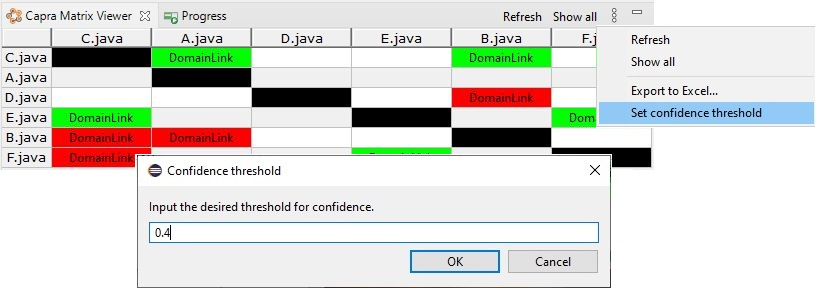
\includegraphics[width=.85\linewidth]{images/matrixViewerExt.JPG}
	\caption{Link representation with uncertainty in matrix view}
	\label{fig:matrixext}
\end{figure}



\subsection{Capra change impact}
Regression tests pass - but we have no serious knowledge on the granularity and coverage of them. We must also mention that we only changed Capra by \textit{adding} new structural features to its core. The impact should be contained (as developers always say).

A further integration of Trace\textit{a} has an impact on Capra. For now, the integration did not require complex changes in the source code, but packages \ughu{ui, core, and persistence had some changes.} It is hazardous to add more specific features to the metamodel for now. The propagation of confidence and the graphical representation of it have been posted in a \ughu{pull request to integrate Trace\textit{a} into Capra's branding}. Before going any further, it is required to bundle them together to benefit from Capra's maintenance.

\subsection{Future work}
This work is a proof-of-concept. On the one hand, it shows the adaptability of Trace\textit{a} and the value of its concepts. The integration works.   
Yet to operationalize Capra would require an upgrade of Capra's main design structure. The \textit{singleton syndrome} needs be addressed.  
